\subsection{Positive Brake Test}\label{sec:braketest_pos}
This test examines the time each motor takes to brake, after it has been instructed to move a full rotation of 360\degree\ in a clockwise direction. The result is given by the number of degrees the motor has moved further than the instructed 360\degree.

\subsection{Hypothesis} 
If a motor is set to move clockwise 360\degree\ and then instructed to brake, the motor will stop without passing the 360\degree\ mark.

\subsection{Test Procedure}
Before performing the test the motors is placed such that they are stable and will therefore be less affected by the environment. Thereafter the motor is connected to the \gls{nxt} which will execute the test software and sample 100 test results automatically, then the test conductor will write down the results and start the next test with a new motor.

The order which the test is performed is:
\begin{enumerate}
  \item Transfer the test software to the \gls{nxt} brick
  \item Place the test motor on a stable surface
  \item Connect test motor to the \gls{nxt} brick
  \item Check that the surface is stable and level
  \item Check that the motor is fasten to the surface
  \item Execute the test software once
  \item When the test program is done, note down the results
\end{enumerate}

\subsection{Data Analysis}
The collected data is represented in \cref{fig:td_brake} and \cref{fig:cmp_all}. The analysis will examine the consistency and standard deviation of the motors. Consistency is measured by how far between the results are form each other when looking at the data from each motor. A motor which has all of its 100 results in the same angle, speaks for a high consistency whereas a motor with 100 results spread amongst 100 different angles shows a low consistency.

\begin{figure}[!htb]
    \centering
    \begin{minipage}{.5\textwidth}
        \centering
        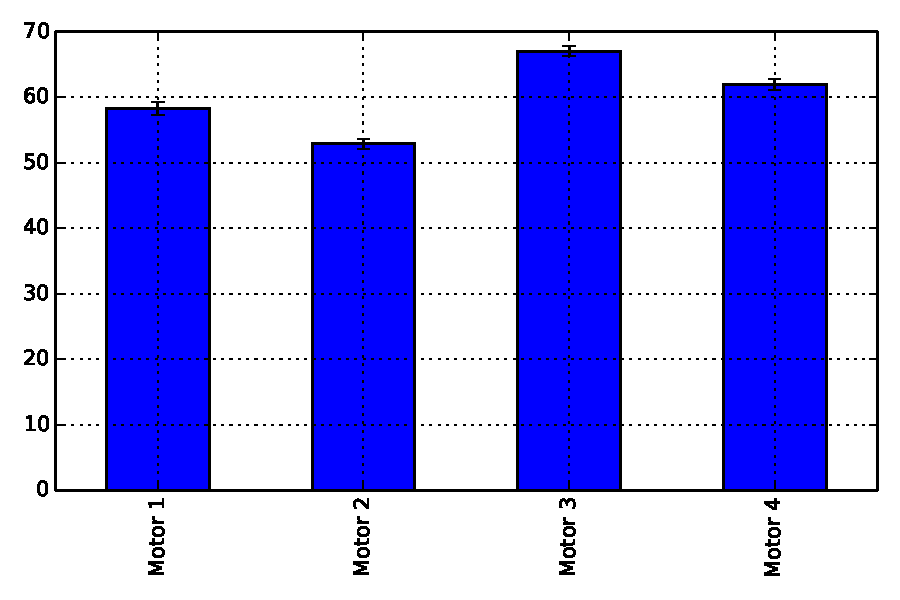
\includegraphics[width=1\textwidth]{graphics/test_graphs/Break_barplot.pdf}
        \caption{Test average for the braking tests}
        \label{fig:td_brake}
    \end{minipage}%
    \begin{minipage}{0.5\textwidth}
        \centering
		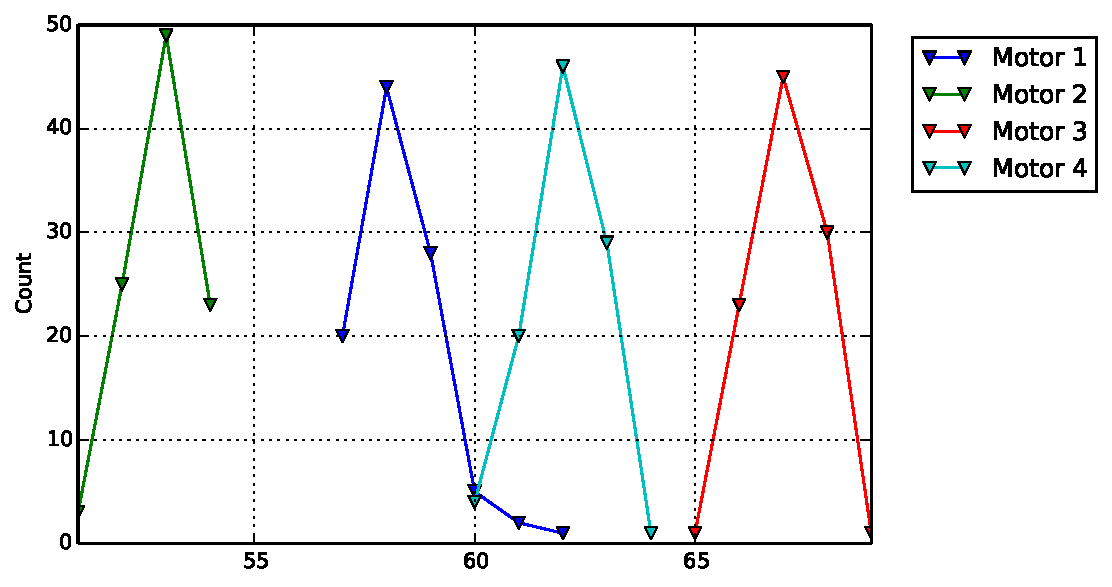
\includegraphics[width=1\textwidth]{graphics/test_graphs/Break_lineplot.pdf}
     	\caption{Test data for motors, with the test \emph{Positive Brake Test}}
		\label{fig:cmp_all}
    \end{minipage}
\end{figure}

Motor 1 is the only graph in  \cref{fig:td_brake} which has more than 4 peeks which makes it more inconsistent than the other motors. According to \cref{tbl:cmpl_test_data} motor 2 and 3 are the most consistent as 97\% and 98\% of the results is 1\degree\ $+-$ from their highest peek.

\begin{table}
  \centering
  \begin{tabular}{| c | c | }
    \hline
    Motor Id & deviation   \\ \hline
    1 & 0.9752492558892912 \\ \hline
    2 & 0.77433581835657   \\ \hline
    3 & 0.7818005635893838 \\ \hline
    4 & 0.83430246677216   \\ \hline
  \end{tabular}
  \caption{The standard deviation for the positive brake test}
  \label{tbl:test_deviation_brake_positive}
\end{table}   

The results are accepted on the basis that the standard deviation is low enough, between 0.77 and 0.98, which supports the integrity of the test as the deviation is below the test resolution of 1\degree . The deviations can be seen in \cref{tbl:test_deviation_brake_positive}. Besides having the largest pool of different end results, motor 1 also has the highest standard deviation, which further supports its exclusion. Motor 2 and 3, again, has the best results as they represent the lowest standard deviation in the test. 

The uncertainties presented in \cref{sec:tech_uncertain}, could have affected the results for the test. Especial the uncertainty concerning \emph{Internal components} as it is central to this test situation. This is due to the fact that to measure the amount of degrees a motor has moved, the motor itself tells how many degrees it has moved. By such the test relies on that the internal motor components measurements are correct and if the internal components are incorrect this can affect the results of the test. 

\subsection{Conclusion of Positive Brake Test}
The hypothesis is not met as all of the motors went above the 360\degree\ mark. It can be concluded that the motors are not able to stop instantaneously after being prompted to brake, but the test shows that the motors perform differently. The best motors, based on consistency and standard deviation from this test, is motor 2 and 3.

\subsection{Negative Brake Test}\label{sec:braketest_neg}
This test examines the time each motor takes to brake, after it has been instructed to move a full rotation of 360\degree\ in a counter-clockwise direction. The result is given by the number of degrees the motor has moved further than the instructed 360\degree .

\subsection{Hypothesis} 
If a motor is set to move counter-clockwise 360\degree\ and then instructed to brake, the motor will stop without passing the 360\degree\ mark.

\subsection{Test Procedure}
Before performing the test the motors is placed such that they are stable and will therefore be less affected by the environment. Thereafter the motor is connected to the \gls{nxt} which will execute the test software and sample 100 test results automatically, then the test conductor will write down the results and start the next test with a new motor.

The order which the test is performed is:
\begin{enumerate}
  \item Transfer the test software to the \gls{nxt} brick
  \item Place the test motor on a stable surface
  \item Connect test motor to the \gls{nxt} brick
  \item Check that the surface is stable and level
  \item Check that the motor is fasten to the surface
  \item Execute the test software once
  \item When the test program is done, note down the results
\end{enumerate}

\subsection{Data Analysis}
The collected data is represented in \cref{fig:td_negative_brake} and \cref{fig:cmp_all_negative}. The analysis will examine the consistency and standard deviation of the motors. Consistency was explained in the Data Analysis section in \cref{sec:braketest_pos}.

\begin{figure}[!htb]
    \centering
    \begin{minipage}{.5\textwidth}
        \centering
        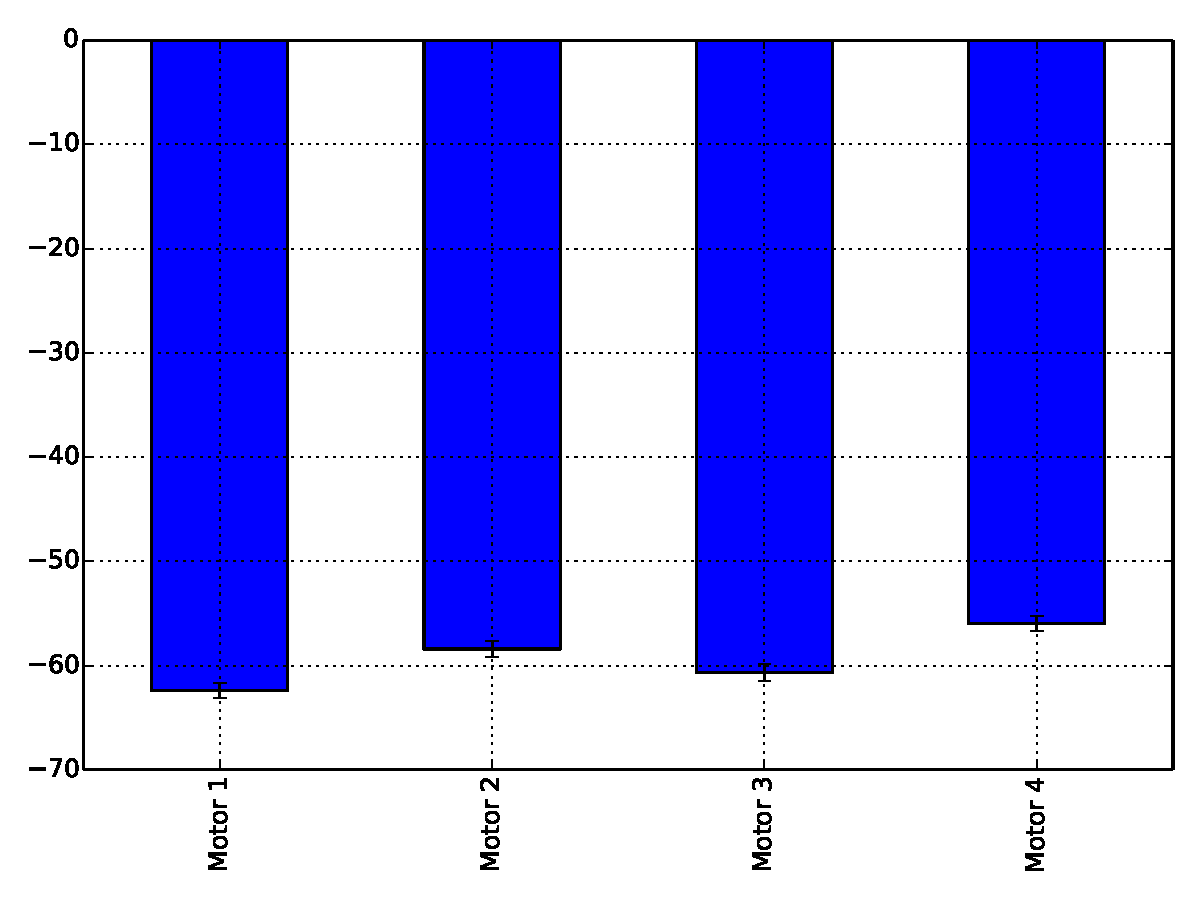
\includegraphics[width=1\textwidth]{graphics/test_graphs/Break_negative_barplot.pdf}
        \caption{Test average for the negative braking tests}
     	\label{fig:td_negative_brake}
    \end{minipage}%
    \begin{minipage}{0.5\textwidth}
        \centering
		 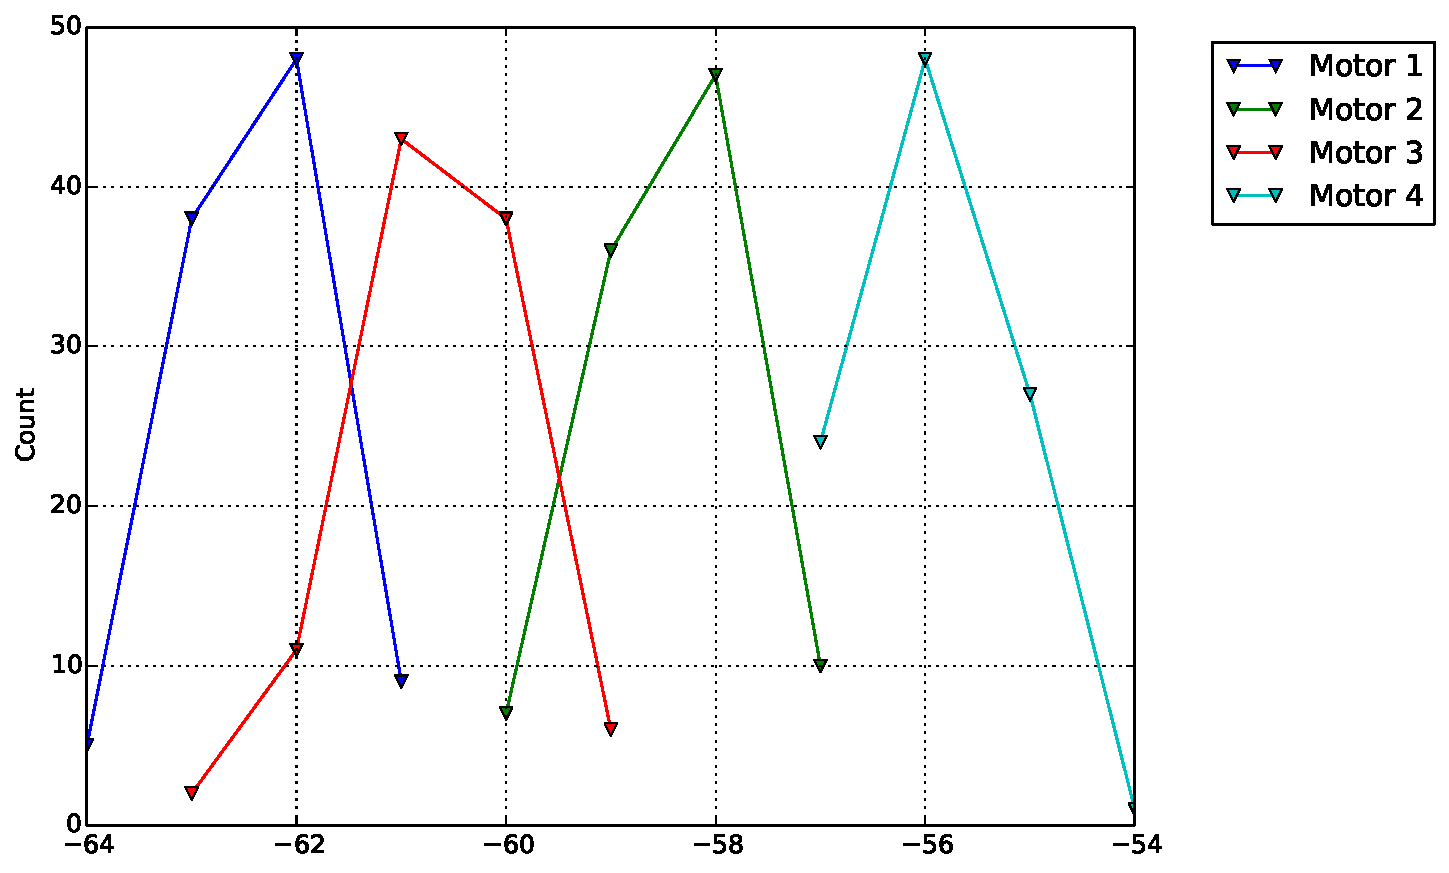
\includegraphics[width=1\textwidth]{graphics/test_graphs/Break_negative_lineplot.pdf}
		 \caption{Test data for four motors, with the test \emph{Negative Brake Test}}
		 \label{fig:cmp_all_negative}
    \end{minipage}
\end{figure}

Motor 3 is the only graph in  \cref{fig:td_negative_brake} which has more than 4 peeks which makes it more inconsistent than the other motors. According to \cref{tbl:cmpl_negative_test_data} motor 1 and 4 are the most consistent as 95\% and 99\% of the results is 1\degree\ $+-$ from their highest peek.

\begin{table}
  \centering
  \begin{tabular}{| c | c | }
    \hline
    Motor Id & deviation   \\ \hline
    1 & 0.7232781713298709 \\ \hline
    2 & 0.7654139963827327 \\ \hline
    3 & 0.8333333333333334 \\ \hline
    4 & 0.7436600722307894 \\ \hline
  \end{tabular}
  \caption{The standard deviation for the positive brake test}
  \label{tbl:test_deviation_brake_negative}
\end{table}   

The results is accepted on the basis that the standard deviation is low enough, between 0.73 and 0.84, which supports the integrity of the test as the deviation is below the test resolution of 1\degree. The deviations can be seen in \cref{tbl:test_deviation_brake_negative}. Besides having the largest pool of different end results, motor 3 also has the highest standard deviation, which further supports its exclusion. Motor 1 and 4, again, has the best results as they represent the lowest standard deviation in the test. 

\subsection{Conclusion of Negative Brake Test}
The hypothesis is not met as all of the motors went above the 360\degree\ mark. It can be concluded that the motors are not able to stop instantaneously after being prompted to brake, but the test shows that the motors perform differently. The best motors, based on consistency and standard deviation from this test, is motor 1 and 4.

\subsection{Conclusion of Acceleration Test}
